% ======================= Pre-Amble =========================
      
%Format
\documentclass[11pt, oneside]{article}   	% use "amsart" instead of "article" for AMSLaTeX format 
                     						%imports package {article} and specify option(s) [11, ai, Essence79pt, oneside]
\usepackage{geometry}                		% See geometry.pdf to learn the layout options. There are lots. 
    \geometry{letterpaper}                   		% ... or a4paper or a5paper or ... 
    %\geometry{landscape}                		% Activate for rotated page geometry

\usepackage[parfill]{parskip}    		        % Activate to begin paragraphs with an empty line rather than an indent

    %Colours
    \usepackage{graphicx, subcaption}
    \usepackage[usenames, dvipsnames]{color}     % font colour:    \textcolor{<colour>}{text}
          									%highlight text:  \colorbox{<color>}{text}
    \usepackage{soul}						%highlight text: \hl{}     %only  yellow								
    									%list of colours: https://www.sharelatex.com/learn/Using_colours_in_LaTeX
    									
    %Bullets
    \usepackage{enumerate}     %specify type of enumeration: \being{enumerate}[<type of enumeration>]
    
    %Footnote Spacing
    \setlength{\footnotesep}{0.4cm}                  %specify spacing b/w footnotes
    \setlength{\skip\footins}{0.6cm}                    % space b/w footnotes and textbody

	%Sections
%	\makeatletter
%	% we use \prefix@<level> only if it is defined
%	\renewcommand{\@seccntformat}[1]{
%	  \ifcsname prefix@#1\endcsname
%	    \csname prefix@#1\endcsname
%	  \else
%	    \csname the#1\endcsname\quad 
%	  \fi}
%	% define \prefix@section
%	\newcommand\prefix@section{Question \thesection}
%	\makeatother

%	\makeatletter
%	\def\@seccntformat#1{%
%	  \expandafter\ifx\csname c@#1\endcsname\c@section
%	  Question \thesection
%	  \else
%	  \csname the#1\endcsname\quad
%	  \fi}
%	\makeatother



%Mattematics
    %American Mathematics Society packages
    \usepackage{amsmath}	   %math
    \usepackage{amssymb}       %symbols
    \usepackage{amsthm}          %theorems
    \newtheorem{proposition}{Proposition}

    %QED
    \newcommand*{\QEDA}{\hfill\ensuremath{\blacksquare}}         %make qed filled square:    \QEDA
    \newcommand*{\QEDB}{\hfill\ensuremath{\square}}               %make qed empty square: \QEDB 
    \renewcommand\qedsymbol{\ensuremath{\blacksquare}}		%Proof environment
    
    % Proofs
	\newtheorem{thm}{Theorem}[section]
	\newtheorem{lem}[thm]{Lemma}
	\newtheorem{prop}[thm]{Proposition}
	\newtheorem*{cor}{Corollary}
	
	\theoremstyle{definition}
	\newtheorem{defn}{Definition}[section]
	\newtheorem{conj}{Conjecture}[section]
	\newtheorem{exmp}{Example}[section]
	
	\theoremstyle{remark}
	\newtheorem*{rem}{Remark}
	\newtheorem*{note}{Note}
	
	% Symbol Shortcuts
	\newcommand{\R}{\ensuremath{\mathbb{R}}}
	\newcommand{\C}{\ensuremath{\mathbb{C}}}
	\newcommand{\Z}{\ensuremath{\mathbb{Z}}}
	\newcommand{\Q}{\mathbb{Q}}
	\newcommand{\N}{\mathbb{N}}
	
	% Augmented Matrix
	\makeatletter
	\renewcommand*\env@matrix[1][*\c@MaxMatrixCols c]{%
  	\hskip -\arraycolsep
 		 \let\@ifnextchar\new@ifnextchar
 		 \array{#1}}
	\makeatother
	
    %\numberwithin{counterA}{counterB} 	% replaces counterA by counterb.countera
	%\numberwithin{equation}{question} 	% for equations: (5) -> (6.1)
    
    % Spacing Units
	\usepackage{siunitx}				% Syntax: \SI{value}{unit}
								%	-> e.g. $\SI{-9.81}{ms^{-2}}$
	
%    % MATLAB in sentence (need mcode.sty in folder)
%	\usepackage[]{mcode} % http://www.mathworks.com/matlabcentral/fileexchange/8015-m-code-latex-package
%	% Syntax:
%	%	- In Sentence: \mcode{<code>}
%	%	- Block of code: \begin{lstlisting} <code> \end{lstlisting}
%	%	- Footnote: \footnote{ \mcodefn{ <code> } }
%	%	- External m-file
%	%		-> Entire file: \lstinputlisting{/SOME/PATH/FILENAME.M}
%	%		-> Certain lines (i.e. skip header): \lstinputlisting[firstline=6, lastline=15]{/SOME/PATH/FILENAME.M}



%Figures
\usepackage{caption}
\captionsetup[figure]{labelfont=bf}    %make figure labels boldface
\captionsetup[table]{labelfont=bf}     %make table labels boldface

\usepackage[hidelinks]{hyperref}                % Allows for clickable references

    %Tables
    \usepackage[none]{hyphenat}                    % Stops breaking-up words in a table (i.e. no hyphens)                                                             
    
    \usepackage{array}   
        \newcolumntype{x}[1]{>{\centering\let\newline\\\arraybackslash\hspace{0pt}}p{#1}}       %center fixed column width: x{<len>}                      
        \newcolumntype{$}{>{\global\let\currentrowstyle\relax}}                                 % let us apply things (e.g. bold/italicize) to entire row            
        \newcolumntype{^}{>{\currentrowstyle}}
        \newcommand{\rowstyle}[1]{\gdef\currentrowstyle{#1} #1\ignorespaces}
    
    %Images
    \graphicspath{ {images/} }                          %directory that your images are located in within your current directory
    
    %Diagrams
    \usepackage[latin1]{inputenc}
    \usepackage{tikz}
    	\tikzset{line/.style={-latex'}}
        \usepackage{tkz-berge}
        \usetikzlibrary{shapes,arrows}
        \usetikzlibrary{patterns}			%Specify colours of stuff (e.g. vertices): 
        										%	-> set style: \tikzset{VertexStyle/.append style = {minimum size = 8pt, inner sep = 0pt}} 
											%	-> change individual vertices: \AddVertexColor{white}{1,2} 


%Bibliography
\usepackage[numbers,sort&compress]{natbib}   %for multiple references: sorts  (i.e. [1,2] NOT [2, 1] )
                                           				  %                                     compresses (i.e. [1-3] )
\usepackage[nottoc]{tocbibind}                            %add bibliography to table of contents


%Miscellaneous
\usepackage{dirtytalk}    %quotations: use \say  
\usepackage{wasysym} 	 % \smiley{} \frownie{} \blacksmiley{}

% ======================== Document ======================
\begin{document}

% Implementation of a Database Management System for The Dempster Carte
\title{Project Proposal\\
\vspace{.4cm}
\large
Group Name: The Dempster Cartel \\
\line(1,0){360} \\               %(slope x, y){length of line}
\vspace{1cm}
\large
The University of British Columbia \\
CPSC 304 \\
September 27, 2016
\vspace{1cm}}


\author{
Knill, Stephanie\\
54882113\\
k0g0b
\and
Lai, Essence\\
29579133 \\
h7x9a
\and
Lin, Terry\\
14558143 \\
h3b0b
}

\date{}                    % Activate:  display a given date (e.g. {August 4} ) or no date (empty {} )
                                    %No activate: display current date
\maketitle

%\begin{abstract}
%Following the classification system employed by Peng et al. (2009), courting behaviour will be recorded if either panda (1) approaches a sexual partner forwardly, presenting estrous or rutting behaviors, such as shaking head, urinating/defecating, rubbing gentile, etc.; (2) bleats ''Mie, Mie'', stares at the partner, sniffs the partner's urine, feces, or the leftover scent mark; or (3) scratches the partner in order to attract his or her attention. Additionally, a successful copulation will be recorded if the male panda's penis penetrates the female panda's vagina and at a latter time a high chirp cry from the female is heard; a failed copulation will be recorded if the keeper has to separate the two pandas because they bit or attacked each other, seldom approached each other in the pen, or display waning courtship. 
%\end{abstract}

\thispagestyle{empty}    %do not display page number on this page


% ================= Table Of Contents ================
\cleardoublepage
\tableofcontents

\thispagestyle{empty}   %do not display page number on this page




% ================= Background/Relevance ================

\cleardoublepage
\setcounter{page}{1}    %set page number to 1 (b/c want to start on first page of contents)

\section{Proposal}
\subsection{Project Description}
The aspects of the drug trade that we will be modelling will be the information relevant to the various transactions and interactions between drug lords, dealers, suppliers and addicts. This includes things like transaction records between suppliers and drug lords, transaction records between dealers and addicts, and the total amount of drugs and money that drug lords have in different territories.

There will be 2 classes of users for our database: drug lords and dealers. A druglord distributes cocaine to his dealers in different territories. Druglords also deal with suppliers directly for cocaine supply. A drug lord can have no suppliers, dealers, and does not oversee any deals (not a very efficient drug lord but it is allowed). Druglords can add themselves to the database and can also remove themselves/other druglords. Dealers sell cocaine to the addicts and reports to their corresponding drug lord regarding the status (i.e. money and drugs) of the territory. Dealers (and druglords) can add/remove addicts from the database as needed.  Every dealer must report to a single dealer and can only belong to one single territory. Dealers cannot add or remove themselves to the database, this can only be done by the drug lord they work under.

Drug lords know everything about the supply transactions and distribution transactions, whereas the dealers only know about distribution transactions. Both types of transaction must involve a drug lord. More specifically, supply transaction is a record of the supply deal between a drug lord and a supplier. Distribution transaction is a record of the day-to-day deals between a dealer and an addict that is overseen by a drug lord. 

This project will be done using the CS department's oracle database and using PHP. We do not anticipate using any special software or hardware.

\cleardoublepage
\subsection{E/R Diagram}

\begin{figure}[h]
\begin{center}
	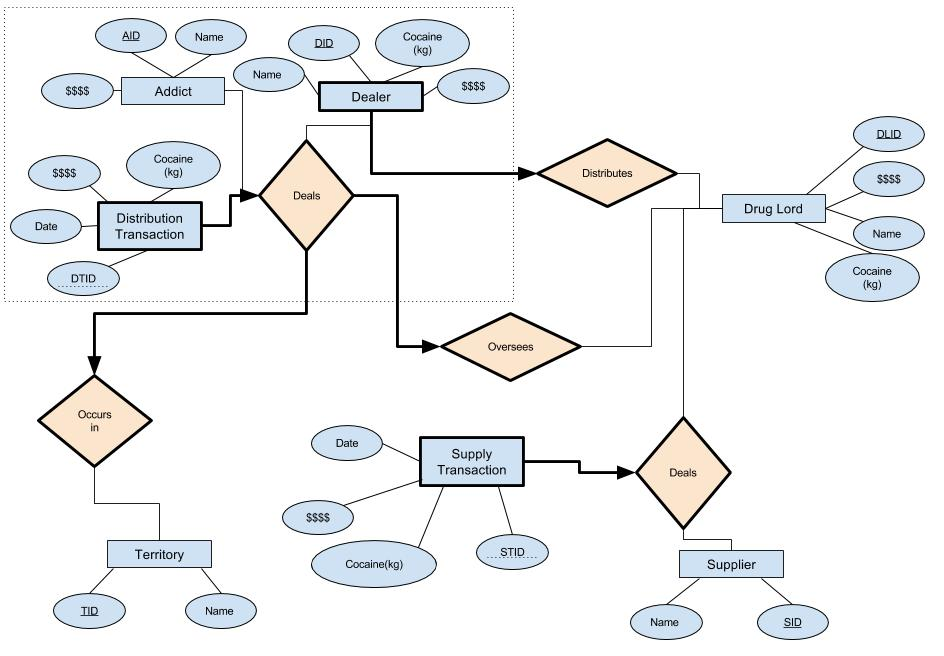
\includegraphics[width=.9\textwidth]{ER_Diagram.jpg}
\end{center}
\end{figure}


\subsection{Application Specifications}
\begin{enumerate}

	\item Make Distribution Transaction
	\begin{itemize}
		\item \textbf{User:} Dealer
		\item \textbf{Input:} Dealer id (\underline{DID}), Addict id (\underline{AID}), Money Exchanged (\$\$\$\$), Drug Amount (Cocaine), and Date
		\item \textbf{Output:} \say{Transaction Completed}, \say{Failure to add Addict to database. Transaction has been aborted.}, \say{Account Does Not Exist}, \say{Insufficient Funds} or \say{Insufficient Drugs}
		\item \textbf{Basic Case:} The system will calculate the total monetary value based on the amount of drugs purchased. If all goes well, the dealer's drug and money supply will be adjusted and the transaction will be added to the Distribution Transaction database and returns \say{Transaction Completed}.
		\item \textbf{Exceptions:}
		\begin{enumerate}
			\item If the Dealer is not in the database, transaction is aborted and \say{Account Does Not Exist} is returned
			\item If the Addict name is not in the database, the system will ask to add the Addict info first, and then will continue. If Addict addition is not successful, transaction is aborted and \say{Failure to add Addict to database. Transaction has been aborted.} is returned.
			\item If there are not enough drugs in Dealer supply, transcation is aborted and \say{Insufficient Drugs} is returned.
			\item If not enough cash is tendered, transaction is aborted and \say{Insufficient Funds} is returned\footnote{And addict is subsequently removed from the database}.
		\end{enumerate}
	\end{itemize}
		
			
	\item Make Supply Transaction
	\begin{itemize}
			\item \textbf{User:} Drug Lord
			\item \textbf{Input:} Drug Lord id (\underline{DLID}), Supplier id (\underline{SID}), Money Exchanged (\$\$\$\$), Drug Amount (Cocaine), and Date
			\item \textbf{Output:} \say{Transaction Completed}, \say{Cancelled}, or \say{Account Does Not Exist}.
			\item \textbf{Basic Case:} The system will calculate the total monetary value based on the amount of drugs purchased. If all goes well, the drug lords's drug and money supply will be adjusted and the transaction will be added to the Distribution Transaction database and returns \say{Transaction Completed}.
			\item \textbf{Exceptions:}
			\begin{enumerate}
				\item If the Drug Lord is not in the database, transaction is aborted and \say{Account Does Not Exist} is returned
				\item If the Supplier name is not in the database, the system will ask to add the Supplier info first, and then will continue. If Supplier addition is not successful, transaction is aborted and \say{Cancelled} is returned.
				\item If there is not enough money in Drug Lord supply, transcation is aborted and "Cancelled" is returned.
			\end{enumerate}
		\end{itemize}	
		
		
	\item View Distribution Transactions
	\begin{itemize}
			\item \textbf{User:} Drug Lord and Dealer.
			\item \textbf{Input:} Dealer id (\underline{DID}), Addict id (\underline{AID}), and/or Distribution Transaction id (\underline{DTID}).
			\item \textbf{Output:} List of transactions involving all given fields, \say{No such transactions exist}, or \say{Account Does Not Exist}, \say{Access Denied}.
			\item \textbf{Basic Case:} If only a user id is given (either a Drug Lord or Dealer id), then all transactions made by the user is displayed. If additional fields are given as input, then only the transactions pertaining to them will be displayed (if user id is granted visibility).
			\item \textbf{Exceptions:}
			\begin{enumerate}
				\item If either the Dealer or Addict id does not exist in the database, transaction is aborted and \say{Account Does Not Exist} is returned.
				\item If the Distribution Transaction id does not exist in the database, transaction is aborted and \say{No such transactions exist} is returned.
				\item If a Dealer tries to access transaction that do not involve said Dealer (i.e. Dealer $i$ tries to view transactions made by Dealer $j$, where $i\neq j$), then \say{Access Denied} is returned.	
				\item If a Drug Lord tries to access transaction that do not involve said Drug Lord (i.e. a Drug Lord from Territory $i$ tries to access transactions from a Territory $j$, where $i\neq j$), then \say{Access Denied} is returned.	
			\end{enumerate}
		\end{itemize}	
	
	
	\item View Supply Transactions
	\begin{itemize}
			\item \textbf{User:} Drug Lord
			\item \textbf{Input:} Drug Lord id (\underline{DLID}), Supplier id (\underline{SID}), and/or  Supply Transaction id (\underline{STID})
			\item \textbf{Output:} List of transactions involving all given fields, \say{No such transactions exist}, or \say{Account Does Not Exist}, \say{Access Denied}.
			\item \textbf{Basic Case:} If only a Drug Lord id is given, then all supply transactions made by them is displayed. However, adding the additional field Supplier id will limit it to only transactions made with a specific supplier, while a Supply Transaction id displays only that transaction.
			\item \textbf{Exceptions:}
			\begin{enumerate}
				\item If either the Drug Lord or Supplier id does not exist in the database, transaction is aborted and \say{Account Does Not Exist} is returned.
				\item If the Supply Transaction id does not exist in the database, transaction is aborted and \say{No such transactions exist} is returned.
				\item If a Drug Lord tries to access transaction that do not involve said Drug Lord (i.e. a Drug Lord from Territory $i$ tries to access transactions from a Territory $j$, where $i\neq j$), then \say{Access Denied} is returned.	
			\end{enumerate}
		\end{itemize}
		
		
	\item View Supply
	\begin{itemize}
		\item \textbf{User:} Drug Lord or Dealer.
		\item \textbf{Input:} Drug Lord (\underline{DLID}) or Dealer id (\underline{DID})
		\item \textbf{Output:} Amount of money (in USD) and cocaine (in kilograms or grams) a Drug Lord or Dealer should have, \say{Account Does Not Exist} or \say{Access Denied}.
		\item \textbf{Basic Case:} If a Drug Lord id is given, then the amount of cash and cocaine the Drug Lord should have is returned. If a Dealer id is given then the amount of cash and cocaine the Dealer should have is returned.
		\item \textbf{Exceptions:}
		\begin{enumerate}
			\item If the Drug Lord or Dealer id is not in the database, transaction is aborted and \say{Account Does Not Exist} is returned.
			\item If a Drug Lord tries to access information about another Drug Lord or Dealer not in his/her territorhy (i.e. a Drug Lord from Territory $i$ tries to access information of a Dealer/Drug Lord from a Territory $j$, where $i\neq j$), then \say{Access Denied} is returned.	
			\item If a Dealer tries to access information about a Drug Lord or any Dealers other than him/herself, then \say{Access Denied} is returned.	
		\end{enumerate}
	\end{itemize}		
			
	
%	\item View Drug Supply
%	\begin{itemize}
%		\item \textbf{User:} Drug Lord or Dealer.
%		\item \textbf{Input:} Drug Lord (\underline{DLID}) or Dealer id (\underline{DID})
%		\item \textbf{Output:} Amount of cocaine a Drug Lord (in kilograms) or Dealer (in grams) should have, \say{Account Does Not Exist} or \say{Access Denied}.
%		\item \textbf{Basic Case:} If a Drug Lord id is given, then the amount of cocaine the Drug Lord should have is returned. If a Dealer id is given then the amount of cocaine the Dealer should have is returned.
%		\item \textbf{Exceptions:}
%		\begin{enumerate}
%			\item If the Drug Lord or Dealer id is not in the database, transaction is aborted and \say{Account Does Not Exist} is returned.
%			\item If a Drug Lord tries to access information about another Drug Lord or Dealer not in his/her territorhy (i.e. a Drug Lord from Territory $i$ tries to access information of a Dealer/Drug Lord from a Territory $j$, where $i\neq j$), then \say{Access Denied} is returned.	
%			\item If a Dealer tries to access information about a Drug Lord or any Dealers other than him/herself, then \say{Access Denied} is returned.	
%		\end{enumerate}
%	\end{itemize}	
%	
%	
%	\item View Money Supply
%	\begin{itemize}
%		\item \textbf{User:} Drug Lord or Dealer.
%		\item \textbf{Input:} Drug Lord (\underline{DLID}) or Dealer id (\underline{DID})
%		\item \textbf{Output:} Amount of money (in USD) a Drug Lord or Dealer should have, \say{Account Does Not Exist} or \say{Access Denied}.
%		\item \textbf{Basic Case:} If a Drug Lord id is given, then the amount of cash the Drug Lord should have is returned. If a Dealer id is given then the amount of cash the Dealer should have is returned.
%		\item \textbf{Exceptions:}
%		\begin{enumerate}
%			\item If the Drug Lord or Dealer id is not in the database, transaction is aborted and \say{Account Does Not Exist} is returned.
%			\item If a Drug Lord tries to access information about another Drug Lord or Dealer not in his/her territorhy (i.e. a Drug Lord from Territory $i$ tries to access information of a Dealer/Drug Lord from a Territory $j$, where $i\neq j$), then \say{Access Denied} is returned.	
%			\item If a Dealer tries to access information about a Drug Lord or any Dealers other than him/herself, then \say{Access Denied} is returned.	
%		\end{enumerate}
%	\end{itemize}	


	\item Transfer Drugs
	\begin{itemize}
		\item \textbf{User:} Drug Lord and Dealer.
		\item \textbf{Input:} Drug Lord id (\underline{DLID}), Dealer id (\underline{DID}), and Drug Amount (Cocaine).
		\item \textbf{Output:} \say{Transaction Completed}, \say{Account Does Not Exist}, or \say{Insufficient Drugs}
		\item \textbf{Basic Case:} If all goes well, both the Dealer and Drug Lord's drug supplies will be adjusted and \say{Transaction Completed} is returned.
		\item \textbf{Exceptions:}
		\begin{enumerate}
			\item If the Dealer or Drug Lord is not in the database, transaction is aborted and \say{Account Does Not Exist} is returned
			\item If there is not enough drugs in the Dealer or Drug Lord's supply, transcation is aborted and \say{Insufficient Drugs} is returned.
		\end{enumerate}
	\end{itemize}
		
	
	\item Transfer Money
	\begin{itemize}
		\item \textbf{User:} Drug Lord and Dealer.
		\item \textbf{Input:} Drug Lord id (\underline{DLID}), Dealer id (\underline{DID}), and Money Exchanged (\$\$\$\$).
		\item \textbf{Output:} \say{Transaction Completed}, \say{Account Does Not Exist}, or \say{Insufficient Funds}
		\item \textbf{Basic Case:} If all goes well, both the Dealer and Drug Lord's money supplies will be adjusted and \say{Transaction Completed} is returned.
		\item \textbf{Exceptions:}
		\begin{enumerate}
			\item If the Dealer or Drug Lord is not in the database, transaction is aborted and \say{Account Does Not Exist} is returned
			\item If there is not enough money in the Dealer or Drug Lord's supply, transcation is aborted and \say{Insufficient Funds} is returned.
		\end{enumerate}
	\end{itemize}
		
	\item Add Drug Lord
	\begin{itemize}
		\item \textbf{User:} Drug Lord
		\item \textbf{Input:} Drug Lord id (\underline{DLID}), Drug Amount (Cocaine), and Money Exchanged (\$\$\$\$).
		\item \textbf{Output:} \say{Drug Lord Added}, or \say{Account Already Exists}.
		\item \textbf{Basic Case:} Drug Lord with a new randomly generate id, name Name, money supply \$0 USD, and cocaine supply  0 kg is added to the database and \say{Drug Lord Added} is returned.
		\item \textbf{Exceptions:}
		\begin{enumerate}
			\item If the Drug Lord is already in the database, addition is aborted and \say{Account Already Exists} is returned.
		\end{enumerate}
	\end{itemize}
		
		
	\item Remove Drug Lord
	\begin{itemize}
		\item \textbf{User:} Drug Lord
		\item \textbf{Input:} Drug Lord id (\underline{DLID})
		\item \textbf{Output:} \say{Drug Lord Removed}, or \say{Account Does Not Exist}.
		\item \textbf{Basic Case:} Drug Lord with given id is removed from the database and \say{Drug Lord Removed} is returned.
		\item \textbf{Exceptions:}
		\begin{enumerate}
			\item If the Drug Lord is not in the database, addition is aborted and \say{Account Does Not Exist} is returned.
		\end{enumerate}
	\end{itemize}
		
	\item Add Dealer
	\begin{itemize}
		\item \textbf{User:} Drug Lord
		\item \textbf{Input:} Dealer id (\underline{DID}), Drug Amount (Cocaine), and Money Exchanged (\$\$\$\$).
		\item \textbf{Output:} \say{Dealer Added}, or \say{Account Already Exists}.
		\item \textbf{Basic Case:} Dealer with given id, money supply \$0 USD, and cocaine supply  0 kg is added to the database and \say{Dealer Added} is returned.
		\item \textbf{Exceptions:}
		\begin{enumerate}
			\item If the Dealer is already in the database, addition is aborted and \say{Account Already Exists} is returned.
		\end{enumerate}
	\end{itemize}
		
	\item Remove Dealer
	\begin{itemize}
		\item \textbf{User:} Drug Lord
		\item \textbf{Input:} Dealer id (\underline{DID})
		\item \textbf{Output:} \say{Dealer Removed}, or \say{Account Does Not Exist}.
		\item \textbf{Basic Case:} Dealer with given id is removed from the database and \say{Dealer Removed} is returned.
		\item \textbf{Exceptions:}
		\begin{enumerate}
			\item If the Dealer is not in the database, addition is aborted and \say{Account Does Not Exist} is returned.
		\end{enumerate}
	\end{itemize}
		
	\item Add Supplier
	\begin{itemize}
		\item \textbf{User:} Drug Lord
		\item \textbf{Input:} Supplier id (\underline{SID})
		\item \textbf{Output:} \say{Supplier Added}, or \say{Account Already Exists}.
		\item \textbf{Basic Case:} Supplier with given id is added to the database and \say{Supplier Added} is returned.
		\item \textbf{Exceptions:}
		\begin{enumerate}
			\item If the Supplier is already in the database, addition is aborted and \say{Account Already Exists} is returned.
		\end{enumerate}
	\end{itemize}
		
		
	\item Remove Supplier
	\begin{itemize}
		\item \textbf{User:} Drug Lord
		\item \textbf{Input:} Supplier id (\underline{SID})
		\item \textbf{Output:} \say{Supplier Removed}, or \say{Account Does Not Exist}.
		\item \textbf{Basic Case:} Supplier with given id is removed from the database and \say{Supplier Removed} is returned.
		\item \textbf{Exceptions:}
		\begin{enumerate}
			\item If the Supplier is not in the database, addition is aborted and \say{Account Does Not Exist} is returned.
		\end{enumerate}
	\end{itemize}
		
		
	\item Add Addict
	\begin{itemize}
		\item \textbf{User:} Dealer, Drug Lord
		\item \textbf{Input:} Addict id (\underline{AID})
		\item \textbf{Output:} \say{Addict Added}, or \say{Account Already Exists}.
		\item \textbf{Basic Case:} Addict with given id is added to the database and \say{Addict Added} is returned.
		\item \textbf{Exceptions:}
		\begin{enumerate}
			\item If the Addict is already in the database, addition is aborted and \say{Account Already Exists} is returned.
		\end{enumerate}
	\end{itemize}
		
	\item Remove Addict
	\begin{itemize}
		\item \textbf{User:} Dealer, Drug Lord
		\item \textbf{Input:} Addict id (\underline{AID})
		\item \textbf{Output:} \say{Addict Removed}, or \say{Account Does Not Exist}.
		\item \textbf{Basic Case:} Addict with given id is removed from the database and \say{Addict Removed} is returned.
		\item \textbf{Exceptions:}
		\begin{enumerate}
			\item If the Addict is not in the database, addition is aborted and \say{Account Does Not Exist} is returned.
		\end{enumerate}
	\end{itemize}
\end{enumerate}


\subsection{Platform(s)}
This project will be done using the CS department's oracle database and using PHP. We do not anticipate using any special software or hardware.




%% ================= Methodology ================
%\cleardoublepage
%\section{Methodology}
%
%
%
%
%% ================= Results ================
%\cleardoublepage
%\section{Results}
%
%
%
%% ================= Discussion ================
%
%\cleardoublepage
%\section{Discussion}
%
%
%
%
%
%% ================= Conclusion ================
%%\cleardoublepage
%%\section{Conclusion}
%
%% ================= Thoughts on the Project ================
%\cleardoublepage
%\section {Thoughts on the Project}



% ================= Bibliography ================
\cleardoublepage

%% Method 1
%\begin{thebibliography}{10}
%
%\bibitem{ref:access} The University of British Columbia. (2015). Access and Diversity. \textit{Student Services}. Vancouver, Canada. $<$http://students.ubc.ca/about/access$>$ Last accessed on 23 November 2015.
%%reference this: \cite{ref:access}
%
%\bibitem{ref:convert} Carter, S. (2015). Mr. Data Converter. \textit{GitHub}. San Francisco, The United States of America. $<$https://goo.gl/f8tOl4$>$ Last accessed on 19 November 2015.
%%reference this: \cite{ref:convert}
%
%\end{thebibliography}
%
%% Method 2
%%\bibliographystyle{IEEEtran}
%%\bibliography{/Users/Stephanie/Documents/School/UBC_this_term/MATH441/Project/references/accessref}  %for bib file, don't write .bib extension
%
%%reference this: \cite{ref:access} or \cite{ref:convert}




% ================= Appendix ================
%\cleardoublepage
%\appendix

%\section{Local Search Code} \label{AppendixA}


\end{document}  